\documentclass{tufte-handout}\usepackage[]{graphicx}\usepackage[]{color}
%% maxwidth is the original width if it is less than linewidth
%% otherwise use linewidth (to make sure the graphics do not exceed the margin)
\makeatletter
\def\maxwidth{ %
  \ifdim\Gin@nat@width>\linewidth
    \linewidth
  \else
    \Gin@nat@width
  \fi
}
\makeatother

\definecolor{fgcolor}{rgb}{0.345, 0.345, 0.345}
\newcommand{\hlnum}[1]{\textcolor[rgb]{0.686,0.059,0.569}{#1}}%
\newcommand{\hlstr}[1]{\textcolor[rgb]{0.192,0.494,0.8}{#1}}%
\newcommand{\hlcom}[1]{\textcolor[rgb]{0.678,0.584,0.686}{\textit{#1}}}%
\newcommand{\hlopt}[1]{\textcolor[rgb]{0,0,0}{#1}}%
\newcommand{\hlstd}[1]{\textcolor[rgb]{0.345,0.345,0.345}{#1}}%
\newcommand{\hlkwa}[1]{\textcolor[rgb]{0.161,0.373,0.58}{\textbf{#1}}}%
\newcommand{\hlkwb}[1]{\textcolor[rgb]{0.69,0.353,0.396}{#1}}%
\newcommand{\hlkwc}[1]{\textcolor[rgb]{0.333,0.667,0.333}{#1}}%
\newcommand{\hlkwd}[1]{\textcolor[rgb]{0.737,0.353,0.396}{\textbf{#1}}}%

\usepackage{framed}
\makeatletter
\newenvironment{kframe}{%
 \def\at@end@of@kframe{}%
 \ifinner\ifhmode%
  \def\at@end@of@kframe{\end{minipage}}%
  \begin{minipage}{\columnwidth}%
 \fi\fi%
 \def\FrameCommand##1{\hskip\@totalleftmargin \hskip-\fboxsep
 \colorbox{shadecolor}{##1}\hskip-\fboxsep
     % There is no \\@totalrightmargin, so:
     \hskip-\linewidth \hskip-\@totalleftmargin \hskip\columnwidth}%
 \MakeFramed {\advance\hsize-\width
   \@totalleftmargin\z@ \linewidth\hsize
   \@setminipage}}%
 {\par\unskip\endMakeFramed%
 \at@end@of@kframe}
\makeatother

\definecolor{shadecolor}{rgb}{.97, .97, .97}
\definecolor{messagecolor}{rgb}{0, 0, 0}
\definecolor{warningcolor}{rgb}{1, 0, 1}
\definecolor{errorcolor}{rgb}{1, 0, 0}
\newenvironment{knitrout}{}{} % an empty environment to be redefined in TeX

\usepackage{alltt}

%\documentclass{article}
\usepackage{graphicx}
%\setkeys{Gin}{width=\linewidth,totalheight=\textheight,keepaspectratio}
% Prints a trailing space in a smart way.
\usepackage{xspace}
\usepackage{hyperref}
\usepackage{amsmath}
\newcommand{\tthdump}[1]{#1}
\usepackage{makeidx}
\usepackage{tabularx}

%\makeindex

\begin{knitrout}
\definecolor{shadecolor}{rgb}{0.969, 0.969, 0.969}\color{fgcolor}\begin{kframe}


{\ttfamily\noindent\color{warningcolor}{\#\# Warning: No security definition has been found for the request}}\begin{verbatim}
## failed to load HTTP resource
\end{verbatim}


{\ttfamily\noindent\bfseries\color{errorcolor}{\#\# Error: 1: failed to load HTTP resource}}\end{kframe}
\end{knitrout}


\title{Buy On Gap trading report - S\&P 500}

\date{ 27 Nov 2013 }

\IfFileExists{upquote.sty}{\usepackage{upquote}}{}


\begin{document}
\maketitle

%\SweaveOpts{concordance=TRUE}
%\setkeys{Gin}{width=1.1\marginparwidth} %% Sweave

\section{Trade execution}
\subsection{Order executed}

% latex table generated in R 3.0.2 by xtable 1.7-1 package
% Thu Nov 28 05:10:20 2013
\begin{table}[ht]
\centering
\begin{tabular}{llrrrrrrr|r}
  \hline
 & Symbol & B.AvgPrc & B.Qty & S.AvgPrc & S.Qty & Profit & Comm. & Return \% & Closing Price \\ 
  \hline
1 & ADI & 47.21 & 2016 & 48.55 & 2016 & 2679.58 & 21.86 & 2.81 & 48.55 \\ 
   \hline
\end{tabular}
\end{table}



\subsection{Stock Portfolio}
% latex table generated in R 3.0.2 by xtable 1.7-1 package
% Thu Nov 28 05:10:20 2013
\begin{table}[ht]
\centering
\begin{tabular}{llrrr}
  \hline
 & Symbol & Quantity & Closing price & Market price \\ 
  \hline
1 & ***NO-ASSET*** &  &  &  \\ 
   \hline
\end{tabular}
\end{table}



\section{Trading Matrix}


% latex table generated in R 3.0.2 by xtable 1.7-1 package
% Thu Nov 28 05:10:20 2013
\begin{table}[ht]
\begin{tabular}{lr}
   \hline
Portofolio Amount: & 97253.40 \\ 
  Asset Amount: & 0.00 \\ 
  Bought Amount: & 95175.36 \\ 
  Sold   Amount: & 97876.80 \\ 
  Commission   : & 21.86 \\ 
  P/L incl Comm: & 2679.58 \\ 
  Ret incl Comm \%: & 2.83 \\ 
  S\&P 500 Ret \%: & 0.25 \\ 
   \hline
\end{tabular}
\caption{The commissions and daily returns are calculated based on the closed position.
The open position is present in the portofolio and assume closing on the next open market.
Portofolio amount is the open order with today closing price.} 
\end{table}



% \section{Trade Slippage}
% 
% <<slippage, echo = FALSE , results='asis'>>=
% 
% colnames(slippage) <- c('Symbol','Open Slippage %', 'Close Slippage %');
% print(xtable(slippage),floating=FALSE,);
% @


\title{Buy On Gap trading report - S\&P 600}
\maketitle

\section{Trade execution}
\subsection{Order executed}


% latex table generated in R 3.0.2 by xtable 1.7-1 package
% Thu Nov 28 05:10:20 2013
\begin{table}[ht]
\centering
\begin{tabular}{llrrrrrrr|r}
  \hline
 & Symbol & B.AvgPrc & B.Qty & S.AvgPrc & S.Qty & Profit & Comm. & Return \% & Closing Price \\ 
  \hline
1 & BRLI & 31.70 & 771 & 29.56 & 771 & -1658.69 & 8.11 & -6.78 & 29.55 \\ 
   \hline
\end{tabular}
\end{table}



\subsection{Stock Portfolio}
% latex table generated in R 3.0.2 by xtable 1.7-1 package
% Thu Nov 28 05:10:20 2013
\begin{table}[ht]
\centering
\begin{tabular}{llrrr}
  \hline
 & Symbol & Quantity & Closing price & Market price \\ 
  \hline
1 & ***NO-ASSET*** &  &  &  \\ 
   \hline
\end{tabular}
\end{table}



\section{Trading Matrix}

% latex table generated in R 3.0.2 by xtable 1.7-1 package
% Thu Nov 28 05:10:20 2013
\begin{table}[ht]
\begin{tabular}{lr}
   \hline
Portofolio Amount: & 97375.84 \\ 
  Asset Amount: & 0.00 \\ 
  Bought Amount: & 24441.34 \\ 
  Sold   Amount: & 22790.76 \\ 
  Commission   : & 8.11 \\ 
  P/L incl Comm: & -1658.69 \\ 
  Ret incl Comm \%: & -1.67 \\ 
  S\&P 600 Ret \%: & 0.67 \\ 
   \hline
\end{tabular}
\caption{The commissions and daily returns are calculated based on the closed position.
The open position is present in the portofolio and assume closing on the next open market.
Portofolio amount is the open order with today closing price.} 
\end{table}



% \section{Trade Slippage}
% 
% <<slippage_sp600, echo = FALSE , results='asis'>>=
% 
% colnames(slippage) <- c('Symbol','Open Slippage %', 'Close Slippage %');
% print(xtable(slippage),floating=FALSE,);
% @

\newpage
\section{News}

%\begin{margintable}

% latex table generated in R 3.0.2 by xtable 1.7-1 package
% Thu Nov 28 05:10:20 2013
\begin{tabularx}{\textwidth}{rX}
  \hline
 & ADI \\ 
  \hline
1 &  Our proven model does not conclusively show that Analog Devices will beat earnings this quarter. That is because a stock needs to have both a positive Earnings ESP and a Zacks Rank \#1, 2 or 3 for this to happen.  \\ 
  2 &  Analog provided a modest outlook for the fourth quarter, with revenues expected in the range of \$675 million to \$700 million, up 2.0\% sequentially.  \\ 
  3 &  Norwood, MA (11/26/2013) - Analog Devices, Inc. (NASDAQ: ADI), a global leader in high-performance semiconductors for signal processing applications, today announced that David Zinsner, Vice President and Chief Financial Officer, and Ali Husain, ...  \\ 
  4 &  Analog Devices, Inc. (NASDAQ: ADI), a global leader in high-performance semiconductors for signal processing applications, today announced financial results for its fiscal fourth quarter and fiscal year which ended November 2, 2013.  \\ 
  5 &  In addition to missing FQ4 revenue estimates (while beating on EPS), Analog Devices (ADI) is guiding for FQ1 revenue to be down 5\%-10\% Q/Q, and for EPS to be in a range of \$0.44-\$0.52.  \\ 
  6 &  Analog Devices Inc. (ADI: Quote) reported fourth quarter adjusted EPS of \$0.62 after the bell Tuesday, up from \$0.58 in the previous year.  \\ 
  7 &  Good afternoon. My name is Krishanda, and I will be your conference facilitator. At this time, I would like to welcome everyone to the Analog Devices Fourth Quarter and Fiscal Year 2013 Earnings Conference Call. [Operator Instructions] Mr. Husain, you ...  \\ 
  8 &  Analog Devices (ADI ) had its price target and estimates trimmed at Jefferies, due to ADI's outlook coming in lower than estimates.  \\ 
  9 &  Analog Devices Inc. (ADI: Quote) reported fourth quarter adjusted EPS of \$0.62 after the bell Tuesday, up from \$0.58 in the previous year.  \\ 
  10 &  Analog Devices, Inc. (NASDAQ:ADI) a company that engages in the design, manufacture, and marketing of analog, mixed-signal, and digital signal processing integrated circuits for use in industrial, automotive, consumer, and communication markets ...  \\ 
   \hline
\end{tabularx}


%\end{margintable}

\newpage
\section{Individual contract}
\begin{fullwidth}
\begin{knitrout}
\definecolor{shadecolor}{rgb}{0.969, 0.969, 0.969}\color{fgcolor}\begin{kframe}


{\ttfamily\noindent\bfseries\color{errorcolor}{\#\# Error: chartSeries requires an xtsible object}}\end{kframe}
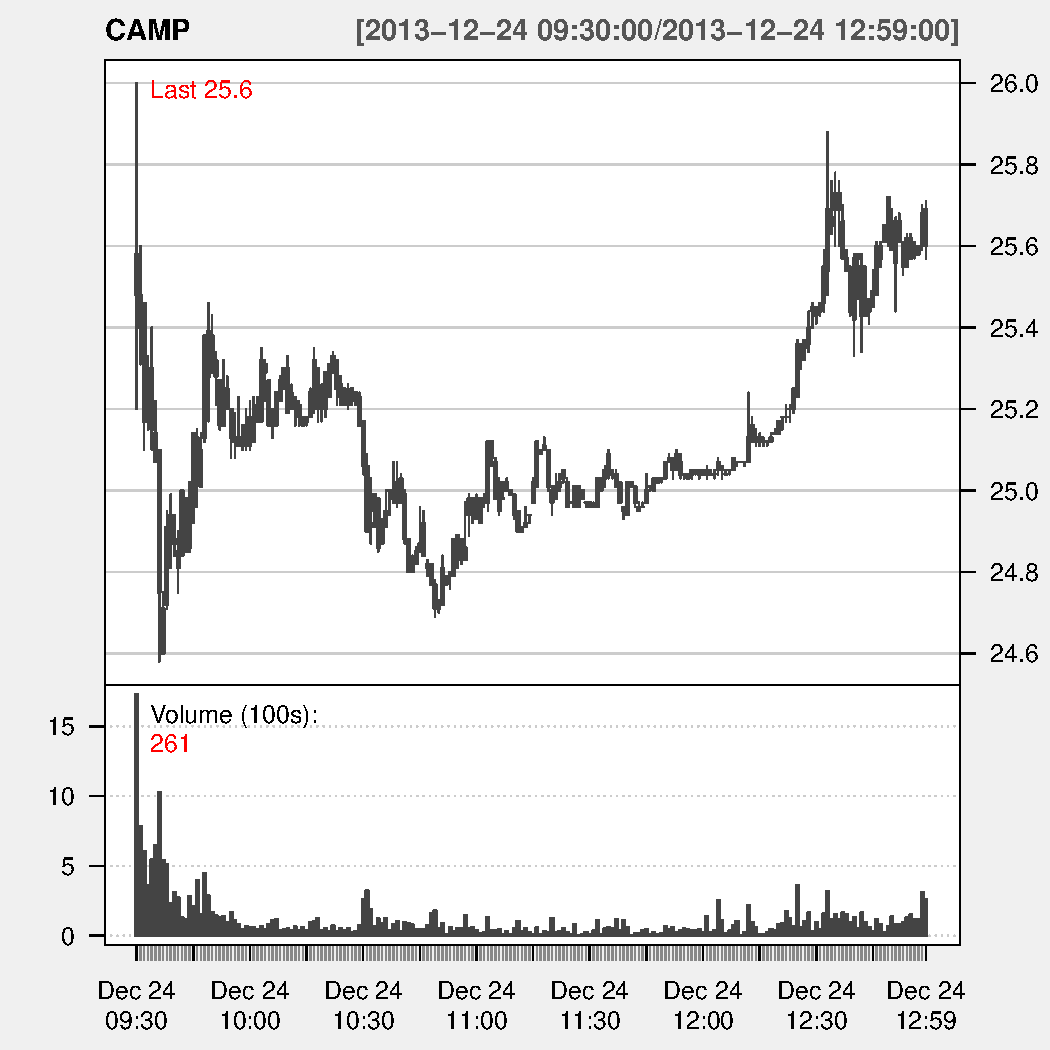
\includegraphics[width=\maxwidth]{/home/jhleong/dev/R/buy_on_gap/BuyOnGap_report/figure/price_chart} 

\end{knitrout}


\end{fullwidth}
\end{document}
